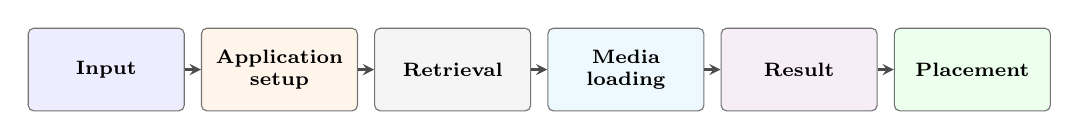
\begin{tikzpicture}[
  phase/.style={draw=black!55, rounded corners=2pt, align=center, minimum height=1.05cm, text width=1.70cm, inner xsep=4pt, font=\scriptsize\bfseries},
  flow/.style={->, thick, draw=black!70},
  >=stealth
]
  \node[phase, fill=blue!7] (input) at (-5.50,0) {Input};
  \node[phase, fill=orange!8] (setup) at (-3.30,0) {Application\\setup};
  \node[phase, fill=black!4] (retrieval) at (-1.10,0) {Retrieval};
  \node[phase, fill=cyan!7] (loading) at (1.10,0) {Media\\loading};
  \node[phase, fill=violet!7] (result) at (3.30,0) {Result};
  \node[phase, fill=green!7] (placement) at (5.50,0) {Placement};

  \draw[flow] (input) -- (setup);
  \draw[flow] (setup) -- (retrieval);
  \draw[flow] (retrieval) -- (loading);
  \draw[flow] (loading) -- (result);
  \draw[flow] (result) -- (placement);
\end{tikzpicture}
